\documentclass[a4j]{jsarticle}

\title{CTRStation数学問題集}
\author{Bamboo}

\usepackage[dvipdfmx]{graphicx}

\begin{document}

\maketitle

\begin{enumerate}
  \setlength{\parskip}{4cm}
  \everymath{\displaystyle}

  \item 図1の外側の円の半径が3のとき,三角形に内接する円の半径を求めよ.(Maru)

  \begin{figure}[htbp]
  \centering
  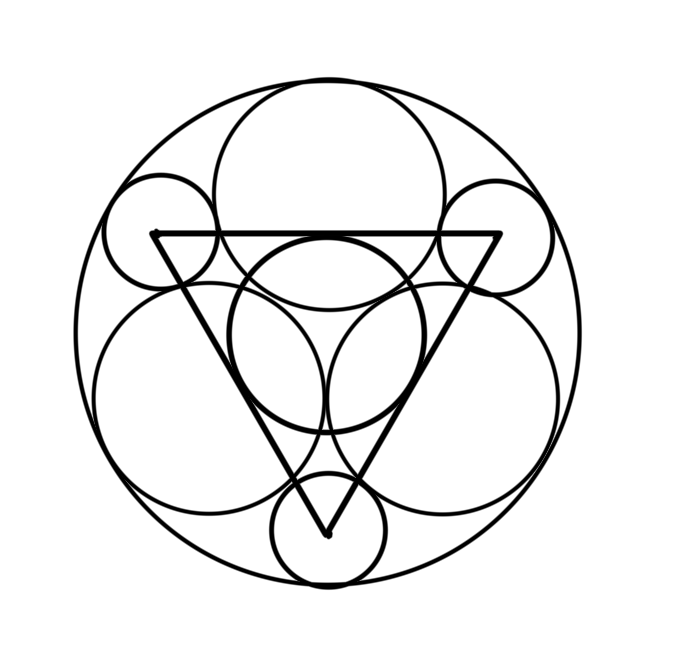
\includegraphics[scale=0.3]{radius.png}
  \caption{}
  \end{figure}

  \item 実数$t$が$0\leq t\leq 1$を動くとき,放物線$y=x^2-\frac{1}{2}t^2x+\frac{1}{3}t^3$の通過領域を図示せよ.(Keito)
  
  \item 広義積分$\int_{0}^{∞}(x-a)^2be^{bx}\,dx$を求めよ.(Bamboo)

\end{enumerate}

\end{document} 